\section[模糊度的LAMBDA解法]{模糊度的LAMBDA解法\\The LAMBDA Method for Ambiguities}
The letters in LAMBDA stand for Least-squares AMBiguity Decorrelation Adjustment. The problem arises in highly accurate positioning by GPS. The carrier phase measurements give a very precise value for the fraction ( in the number of wavelengths from satellite to receiver), but these measurements do not directly yield the integer. For each satellite-receiver pair, the problem is to determine this "ambiguity."Once we find the integer, we can generally track it; a cycle slip is large enough to detect. (Recall that the wavelengths for L1 and L2 are 0.1905m and 0.2445m.) The integer is the problem.

The LAMBDA method was developed by Peter Teunissen (1993-1996). Its MATLAB implementation has been clearly described by de Jonge\&Tiberius (1996). We are grateful to Christian Tiberius for his help in adding the M-files to the library for this book.

The information at our disposal is from phase observations. To remove contamination by clock errors, we generally form double differences: receivers z,j and satellites k,l.The double difference of carrier phase measurements $\Phi(t)$ at a specific time (epoch t) is
\begin{equation}
b_{ij}^{kl}(t)=(\Phi_{i}^{k}(t)-\Phi_{i}^{l}(t))-(\Phi_{j}^{k}(t)-\Phi_{j}^{l}(t))
\end{equation}
The vector b contains m measurements, and the vector I contains the n integer unknowns:
\begin{equation}
I_{ij}^{kl}=(I_{i}^{k}-I_{i}^{l})-(I_{j}^{k}-I_{j}^{l})
\end{equation}
There are other unknowns of great importance! Those are the baseline coordinates $X_{i}-X_{j}$ and $Y_{i}-Y_{j}$ and $Z_{i}-Z_{j}$ that we set out to compute. They are real numbers, not integers, and they go into a vector x with p components. For one baseline p=3. Then the linearized double difference equations are
\begin{equation}
b=Ax+GI+noise
\end{equation}
A is an m by p matrix and G is m by n. The matrix A relates baselines (the coordinate differences in x) to the phase measurements in b. Thus A involves the geometry of positions and lengths, as it does for code observations. The matrix G picks out from each double difference $b_{ij}^{kl}(t)$ the contribution $I_{ij}^{kl}$ from the integers. These ambiguities $I_{ij}^{kl}$ are fixed in time, nominally at their starting values. The other term Ax accounts for all fractions at the start and all phase changes as the observations proceed.

We suppose that enough observations have been made to determine (usually they
overdetermine) x and I. Algebraically, the combined matrix [A G] has full column rank p + n. The ordinary normal equations could be solved, but $\hat{I}$ won�� t contain integers. We are hoping to achieve good precision from a short series of observations. (But not too short.The n observations at one instant are not enough to determine the n integers in I and also the baseline coordinates.)

The covariance matrix $\Sigma_{b}$ of the observations is assumed known. Since differences are correlated,$\Sigma_{b}$ is not at all a diagonal matrix. This is what makes our problem more difficult. This also explains the letter D in LAMBDA, for Decorrelation. The method consists in decorrelating errors (diagonalizing $\Sigma_{b}$, by a change of variables) as far as possible.The limitation is that the change of variables and its inverse must take integers to integers.

The usual problem in weighted least squares is to minimize $||b-Ax-GI||^{2}$. The weighting matrix $\Sigma_{b}^{-1}$ determines the norm, as in $||e||^{2}=e^{T}\Sigma_{b}^{-1}e$. The minimization gives real numbers $\hat{x}$ and $\hat{I}$ (not integers!). This estimate for x and I is called the float solution, and it comes from the ordinary normal equations:
\begin{equation}
\begin{bmatrix}
A & G
\end{bmatrix}^{T}
\Sigma_{b}^{-1}
\begin{bmatrix}
A & G
\end{bmatrix}
\begin{bmatrix}\hat{x}\\\hat{I}
\end{bmatrix}
=
\begin{bmatrix}
A & G
\end{bmatrix}^{T}
\Sigma_{b}^{-1}b.
\end{equation}
We have two block equations, and the left side can be processed first (set $\Sigma_{b}^{-1}=C$):
\begin{equation}
\begin{bmatrix}
A^{T}\\G^{T}
\end{bmatrix}C
\begin{bmatrix}
A&G
\end{bmatrix}
=
\begin{bmatrix}
A^{T}CA & A^{T}CG\\
G^{T}CA & G^{T}CG
\end{bmatrix}
\end{equation}
A block triangular factorization comes from elimination. We are multiplying the upper block row by $G^{T}CA(A^{T}CA)^{-1}$ and subtracting from the lower block row. The new coefficient matrix in the ( 2,2) block is $G^{T}C'G$, with the reduced weight matrix $C'$ exactly as in Section 6.6.3. Elimination of $\hat{x}$ reaches an equation for $\hat{I}$:
\begin{equation}
G_{T}C'G\hat{I}=G^{T}C'b
\end{equation}
When elimination continues, the matrix on the left is factored into $G^{T}C'G=LDL^{T}$. Then ordinary forward elimination and back substitution yield $\hat{I}$. The triangular L(with ones on the diagonal)and the diagonal matrix D are actually the (2,2) blocks in a factorization of the complete matrix in (10.38).

Our problem is that $\hat{I}$ is not a vector of integers.This float solution minimizes a quadratic over all real vectors, while our problem is really one of integer least squares:
\begin{equation}
Minimize\,\,(GI-b)^{T}C'(GI-b)\,\,over\,\, integer\,\, vectors\,\, I.
\end{equation}
The integer solution will be denoted by $\check{I}$ and called the final solution. After $\check{I}$ is found (this is our real problem ), the corresponding $\check{x}$ will come from back-substitution in (10.37):
\begin{equation}
A^{T}CA\check{x}=A^{T}Cb-A^{T}CG\check{I}
\end{equation}
The right side is known , and $A^{T}CA$ on the left side was already factored at the start of elimination. So $\check{x}$ is quickly found.

\subsection{integer Least Squares}

We are minimizing a quadratic expression over integer variables.The absolute minimum occurs at $\hat{I}$; the best integer vector is $\bar{I}$. The coefficient matrix of the second-degree term in (10.40)is $G^{T}C'G$, which is just the (2, 2) block in (10.38) after elimination. For blocks A,B,C, D that (2, 2) block will be $Q = D - CA^{-1}B$. (In mathematics this is called the
Schur complement.) With the blocks that appear in (10.38), this matrix Q is
\begin{equation}
Q = G^{T}CG - G^{T}CA(A^{T}CA)^{-1}A^{T}CG\,\,\,\,\,\,\,\,(which\,\,displays\,\,G^{T}C'G)
\end{equation}

Now consider the minimization for $\bar{I}$. The quadratic expression in (10.40) has its absolute minimum at the float solution $\hat{I}$. Knowing that the coefficient matrix is Q, the problem (10.40) can be stated in a very clear and equivalent form:
\begin{equation}
Minimize\,\,(I-\hat{I})^{T}Q(I-\hat{I})\,\,over\,\, integer\,\, vectors\,\, I.
\end{equation}
This is the problem we study, and one case is especially simple. If Q is a diagonal matrix, the best vector $\bar{I}$ comes from rounding each component of $\hat{I}$ to the nearest integer. The components are uncoupled when Q is diagonal. The quadratic in (10.43) is a sum of squares ,$\Sigma Q_{jj}(I_{j}-\hat{I}_{j})^{2}$. Minimizing each term , the best $\bar{I}_{j}$ is the integer nearest to $\hat{I}_{j}$.

Unfortunately, the actual Q may be far from diagonal. If we could change variables at will, we could diagonalize Q. But we are not completely free , since I is restricted to integers . A change of variables to $J=Z^{-1}I$ is only allowed if Z and $Z^{-1}$ are matrices of integers. Then J is integer exactly when I is integer. The transformed quadratic has absolute minimum at $\hat{J}=Z^{-1}\hat{I}$, and we search for its integer minimum $\bar{J}$:
\begin{equation}
Minimize\,\,(J-\hat{J})^{T}(Z^{T}QZ)(J-\hat{J})\,\,over\,\, integer\,\, vectors\,\,J.
\end{equation}
The search is easier if $Z^{T}QZ$ is nearly diagonal ; its off- diagonal entries should be small.

We can describe in one paragraph the idea behind the choice of Z in the LAMBDA method.��Integer elimination�� will be done in the natural order, starting with the first row of Q. There will certainly be row exchanges, and you will see why. The essential idea was given by Lenstra \& Lenstra \& Lovasz (1982), and the algorithm is sometimes called $L^{3}$. The actual LAMBDA implementation might operate on columns instead of rows, and might go right to left. But to make the following paragraph clear, we just ask ourselves how to create near-zeros off the diagonal with integer elimination.

The first pivot is $Q_{11}$ and the entry below it is $Q_{21}$. Normally we multiply the pivot row the ratio $l_{21}=Q_{21}/Q_{11}$and subtract from the second row. This produces a zero in the (2, 1) position. Our algorithm chooses instead the integer $n_{21}$ that is nearest to $l_{21}$.That choice produces a near-zero in the (2,1) position , not larger than $\frac{1}{2}Q_{11}$:
\begin{equation}
|Q_{12}-n_{21}Q_{11}|=|l_{21}Q_{11}-n_{21}Q_{11}| \leq \frac{1}{2}Q_{11}
\end{equation}

If elimination continues in this usual order, the entry in each off-diagonal (i,j) position
becomes not larger than half of the jth pivot $d_{j}$. Together with the row operations to reduce the subdiagonal , we are including the corresponding column operations to reduce the superdiagonal. This produces a symmetric $Q'=Z_{T}QZ$. The integers $n_{ij}$ yield $Z^{T}$ and Z as products of��integer Gauss steps��like
$$
\begin{bmatrix}
1&0\\
-n_{21}&1
\end{bmatrix}
\,\,\,\,
with \,\, inverse \,\,\,\,
\begin{bmatrix}
1&0\\
n_{21}&1
\end{bmatrix}
$$
So Z and $Z_{-1}$ are integral, and they are assembled in the usual way. But a crucial point is still to be considered: smaller pivots $d_{j}$ lead to smaller off-diagonal entries ($\leq\frac{1}{2}d_{j}$).We prefer a row ordering in which the small pivots come first. The pivots are not known in advance, so the LAMBDA algorithm exchanges rows when a small pivot appears later.Then it recalculates the elimination to achieve ( after iteration ) the desired ordering.

A row exchange comes from a permutation matrix. The ��decorrelating matrices�� Z and $Z^{-1}$ are no longer triangular, but they still contain integers. The new form (10.44) of the minimization has a more nearly diagonal matrix $Q'=Z^{T}QZ$. This greatly reduces the number of candidate vectors J. We display here a typical matrix Z from a specific calculation (and $Z^{-1}$ also contains integers!):
$$
Z=
\begin{bmatrix}
-2&3&1\\
3&-3&-1\\
-1&1&0
\end{bmatrix}\,\,\,\,\,
and\,\,\,\,\,
Z^{-1}=
\begin{bmatrix}
1&1&0\\
1&1&1\\
0&-1&-3
\end{bmatrix}
$$
You can see how $Q'=Z^{T}QZ$ has moved significantly toward a diagonal matrix:
$$
Q=
\begin{bmatrix}
6.290&5.978&0.544\\
5.978&6.292&2.340\\
0.544&2.340&6.288
\end{bmatrix}\,\,\,\,\,decorrelates\,\,to\,\,\,\,\,
Q'=
\begin{bmatrix}
4.476&0.334&0.230\\
0.334&1.146&0.082\\
0.230&0.082&0.626
\end{bmatrix}
$$
The pivots = $(conditional\,\, variances)^{-1}$ for Q and $Q'$ are
$$
\begin{bmatrix}
0.090\\
5.421\\
6.288
\end{bmatrix}\,\,\,\,\,and\,\,\,\,\,
\begin{bmatrix}
4.310\\
1.135\\
0.626
\end{bmatrix}
$$
Notice that LAMBDA reverses the elimination order, up instead of down! The final ambi  -guides are not rounded values of the original float ambiguities $\hat{I}$, but close:
$$
I_{float}=\hat{I}=
\begin{bmatrix}
5.450\\
3.100\\
2.970
\end{bmatrix};\,\,\,\,\,
I_{fixed}=\bar{I}=\begin{bmatrix}
5\\
3\
4
\end{bmatrix}.
$$
$Q'$is more nearly diagonal than Q. The integer least-squares problem (the shortest lattice vector problem) is easier because the ellipsoids $J^{T}Q'J$ = constant are not so elongated .But we still have to search for the $\bar{J}$ that minimizes $(J-\hat{J})^{T}Q'(J-\hat{J})$. We could search in a ball around $\hat{J}$, but the actual LAMBDA implementation is more subtle.

Somewhere the algorithm will factor $Q'$ into $LDL_{T}$. These factors come from elimination , and they indicate search ranges for the different components of J. The off-diagonal entries of L reflect correlation that has not been removed. The search ellipsoid around $\hat{J}$ has its volume controlled by the constant c:
\begin{equation}
(J-\hat{J})^{T}Q'(J-\hat{J})=\sum d_{i}(J_{i}-\hat{J_{i}}+\sum l_{ki}(J_{k}-\hat{J}_{k}))^{2}\leq c^{2}
\end{equation}
de Jonge \& Tiberius (1996) search in backward order $J_{n},...,J_{1}$.When $J_{i}$ is reached, a list of possibilities has been created for all $J_{k}$ with $k > i$ . For each of those possibilities,the bound (10.46) allows a finite search interval (probably small and possibly empty) of integer candidates $J_{i}$. When we reach i=1, a complete candidate vector J satisfying (10.46) has been found. The search ends when all candidates are known.

We chose c large enough to be certain that there is at least one candidate (for example,
$\hat{J}$ rounded to nearest integers). Then there is an efficient recursion to compute $(J-\hat{J})^{T}Q'(J-\hat{J})$ for all candidates.

\subsection{easy12}

easy12 elucidates how the LAMBDA method works on a case with three ambiguities.

Minimizing a Quadratic Expression over Integers The LAMBDA method starts as other
least-squares computations by solving the normal equations (10.37). The result is partly  the vector of real -valued ambiguities $\hat{I}$ and partly the covariance matrix $\Sigma_{\hat{I}}$.

The core problem can be stated in a very clear form
\begin{equation}
Minimize\,\,\,\,(I-\hat{I})^{T}\Sigma_{\hat{I}}^{-1}(I-\hat{I}).
\end{equation}

In one case this problem is especially simple. If $\Sigma_{\hat{I}}^{-1}$ is diagonal, the best vector $\hat{I}_{j}$ comes from rounding each component of $\hat{I}$ to the nearest integer. The components are uncoupled when $\Sigma_{\hat{I}}^{-1}$ is diagonal. The quadratic is a sum of squares $\sum(\Sigma_{\hat{I}}^{-1})_{jj}(I_{j}-\hat{I}_{j})^{2}$.The minimum comes by rounding. Each term in the sum is as small as possible.

In practice the individual $\hat{I}_{j}$ components are highly correlated. Recalling that we often deal with 20 ambiguities, a search procedure to find the minimum is unrealistic.Therefore an idea about decorrelating the ambiguities as much as possible, before starting the search, should lead to an effective procedure.

The first step consists in transforming $\Sigma_{\hat{I}}^{-1}$ such that its off-diagonal entries become numerically smaller. These entries measure the correlation.

We start by computing the $LDL^{T}$ decomposition of the given covariance matrix
$$
\Sigma_{\hat{I}}=LDL^{T}
$$
Next we construct a matrix of integers Z from L by a sequence of integer Gauss transformations and permutations such that
$$
\Sigma_{\bar{I}}=Z^{T}\Sigma_{\hat{I}}Z
$$
is as ��diagonal�� as possible. Now the search defined by (10.47) is substituted by a search over integers I:
\begin{equation}
(I-\hat{I})^{T}Z^{T}\Sigma_{\hat{I}}^{-1}Z(I-\hat{I})=min
\end{equation}
The choice of Z is based on integer elimination starting with the first row of L. This will
certainly involve row exchanges and, therefore, Z will not be triangular. The essential idea for this lattice basis reduction was given by Lenstra, Lenstra, and Lovasz in 1982, and the algorithm is sometimes called $L^{3}$. For further details see Strang \& Borre (1997), pages \textbf{495-499}.

The result of the search is the integer vector $\bar{I}$. Finally, $\bar{I}$ is transformed back to the ambiguity space according to
\begin{equation}
\check{I}=(Z^{-1})^{T}\bar{I}
\end{equation}

Note that both Z and $Z^{-1}$ must have integer entries. A consequence of this is that det(Z) = 1 as seen from Cramer��s rule. The condition on the determinant of Z means that the Z transformation preserves the search volume. At the end of this procedure we have transformed a highly correlated space (elongated ellipsoids) into a sphere-like search space, which diminishes the search time tremendously.

easy12 illustrates the computational steps including a few numerical details. We
choose a numerical example from de Jonge \& Tiberius (1996). Further computational
details are well described in that report.

A Numerical Example Start from the float ambiguities
\begin{equation}
\hat{I}=
\begin{bmatrix}
5.45\\
3.1\\
2.97
\end{bmatrix}
=I_{integer}+\hat{I}_{r}
=\begin{bmatrix}
5\\
3\\
2
\end{bmatrix}+
\begin{bmatrix}
0.45\\
0.10\\
0.97
\end{bmatrix}
\end{equation}

Factor the covariance matrix into
\begin{equation}
\Sigma_{\hat{I}}=
\begin{bmatrix}
6.290&5.978&.544\\
5.978&6.292&2.340\\
.544&2.340&6.288
\end{bmatrix}
=LDL^{T}
\end{equation}
with
\begin{equation}
L=
\begin{bmatrix}
1&0&0\\
1.065&1&0\\
0.087&0.372&1
\end{bmatrix}\,\,\,
and \,\,\,
D=
\begin{bmatrix}
0.090&&\\
&5.421&\\
&&6.288
\end{bmatrix}
\end{equation}
We then compute the $\chi^{2}$ which limits the initial size of the search ellipsoid:
$$
(I-\hat{I})^{T}\Sigma_{\hat{I}}^{-1}(I-\hat{I})<\chi^{2}
$$
it is difficult to determine the initial size of $\chi^{2}$.It must be large enough to include all N-values and on the other hand small to minimize computation time. Often we are also interested in estimating several N-values for each ambiguity. We may need them for testing purposes like in equation (10.56). Obviously $\chi^{2}$ (whose units are $cycles^{2}$) depends on n,and limits the squared distances of partially rounded float vectors to the float vector in the metric of the covariance matrix. In the present example the search volume is determined by $\chi^{2}=1.245$.

The call $[\Sigma_{\bar{I}},Z,L_{t},D_{t}]$ = decorrel($\Sigma_{\hat{I}},\hat{I}_{r}$) computes the integer transformation matrix Z,decorrelated covariance matrix $\Sigma_{\bar{I}}$, and the transformed $D_{t}$ and $L_{t}$:
\begin{equation}
Z=
\begin{bmatrix}
-2&3&1\\
3&-3&-1\\
-1&1&0
\end{bmatrix}\,\,\,\,\,
leads\,\,to\,\,\,\,\,
I_{s}=Z^{T}\hat{I}_{r}=
\begin{bmatrix}
-1.57\\2.02\\0.35
\end{bmatrix}
\end{equation}
The transformed , decorrelated covariance matrix is
\begin{equation}
\Sigma_{\bar{I}}=Z^{T}\Sigma_{\hat{I}}Z=
\begin{bmatrix}
4.476&0.334&0.230\\
0.334&1.146&0.082\\
0.230&0.082&0.626
\end{bmatrix}
\end{equation}

Note the diminished off-diagonal terms! The $L_{t}$ and $D_{t}$$L_{t}$ used in the search are
$$
L_{t}=
\begin{bmatrix}
1.000&0.000&0.000\\
0.268&1.000&0.000\\
0.367&0.131&1.000
\end{bmatrix}\,\,\,
and \,\,\,
D_{t}=
\begin{bmatrix}
4.310&&\\
&1.135&\\
&&0.626
\end{bmatrix}
$$
The search domain is $
(I-\hat{I})^{T}(Z^{T}\Sigma_{\hat{I}}Z)(I-\hat{I})<\chi^{2}
$, for I integer. Determination of the size of the new search volume for $L_{t}$ and $D_{t}$ yields $\chi^{2}$ = 0.218.

The search yields final and fixed ambiguities
$$
\check{I}=
\begin{bmatrix}
5\\3\\4
\end{bmatrix}
$$
We notice that this integer result $\check{I}$ could not be derived from the float values I in (10.50).This is due to the non-zero correlations between the individual ambiguities. With this we end the small numerical example demonstrating the LAMBDA method.

\subsection{When to Fix the Ambiguities?}

Any procedure to estimate ambiguities involves solving normal equations (or applying an
appropriate filter). Normal equations are accumulative and one may ask when to stop the
accumulation and solve the normals? Of course, the $A^{T}A$ matrix must be positive definite before this happens. But how many epochs must be processed before we may obtain a good solution ? In the following we will try to provide a partial answer to the situation.

The LAMBDA method comes with a colossal construction based on the probability
\begin{equation}
P=\prod_{i=1}^{n}(2\Phi(\frac{1}{2\sigma_{\hat{Z}_{i|I}}})-1)=\prod_{i=1}^{n}erf(\frac{1}{2\sqrt{2}\sigma_{\hat{Z}_{i|I}}})
\end{equation}
$\sigma_{\hat{Z}_{i|I}}$ is the conditional standard deviation of the i-th transformed ambiguity, sequentially conditioned on the previous i -1 ambiguities, and
$$
\Phi(x)=\frac{1}{\sqrt{2\pi}}\int_{-\infty}^{x}exp(-\frac{1}{2}z^{2})dz
$$

Depending on the model used , we theoretically can estimate all ambiguities from a few epochs of data. It is always most difficult to fix correctly the first three ambiguities. So one strategy is to take n = 1, compute P for the individual satellites, and select the three satellites with highest probability. Next to take n = 3 and compute the combined P. This value has to be larger than 0.999 before we can estimate any integer successfully.

If P is still too low, we have to add the contribution to the normals $A^{T}CA$ from more epochs before we compute the least-squares solution and again compute the P$-$values. This procedure continues till we have turned all ambiguities into integers.

The following MATLAB code computes P:

function P = success(D);

\%SUCCESS success rate for given ambiguities

n = size(D,2);

P = 1;

for i = 1:n

x = 1/(2*sqrt(D(i)));

P = P*erf(x);

end

This last part can also be done using recursive least squares. Let the ambiguities for an epoch k be captured in the vector $\hat{a}_{k}$, with covariance matrix $\Sigma_{\hat{a}_{k}}$. Assume that the estimate $\hat{a}_{(k-1)}$, with covariance matrix $\Sigma_{\hat{a}_{(k-1)}}$ is available. Then the updated estimate $\hat{a}_{(k)}$ of the ambiguity vector, with its covariance matrix  $\Sigma_{\hat{a}_{(k)}}$, is obtained as
$$
\hat{a}_{(k)}=\Sigma_{\hat{a}_{(k)}}(\Sigma_{\hat{a}_{(k-1)}}^{-1}\hat{a}_{(k-1)}+\Sigma_{\hat{a}_{(k)}}^{-1}\hat{a}_{(k)})
$$
$$
\Sigma_{\hat{a}_{(k)}}=(\Sigma_{\hat{a}_{(k-1)}}^{-1}+\Sigma_{\hat{a}_{(k)}}^{-1})^{-1}
$$
Since this covariance matrix is ��smaller�� than the one based on a single epoch of data,
the resulting probability of correctly fixing the integer ambiguities will be larger. This
accumulation of normal equations is repeated until P $>$ 0.999.

\begin{figure}
	\centering
	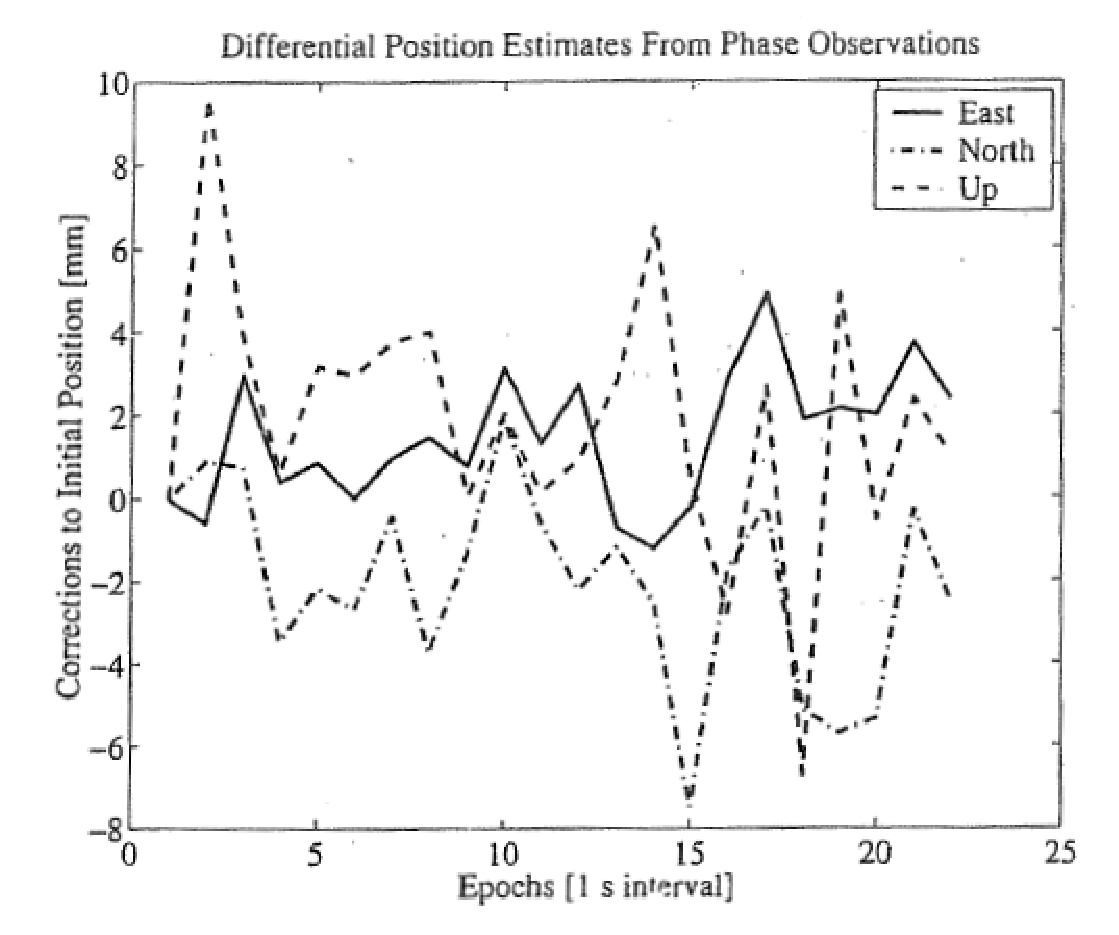
\includegraphics[width=0.4\linewidth]{TeX_files/Part03/chapter10/image/9-8}
	\caption{Baseline over time from pseudoranges and phases at two receivers}
	\label{fig:9-8}
\end{figure}

Once the integer values of the ambiguities have been determined, they can be transicrred to subsequent epochs, provided no loss of lock or cycle slip occurs.

In case of loss of lock or cycle slip, the ambiguities for the satellite(s) concerned must be estimated again. If the integer ambiguities of at least three of the remaining satellites have already been determined, then usually one epoch is sufficient to estimate all ambiguities with a success rate close to 100\%.

To judge the quality of the estimated integer ambiguities, the LAMBDA software outputs
two integer solutions, $\check{a}_{best}$ and $\check{a}_{2nd\,\,best}$.The best solution is the one which minimizes
$$
(\hat{a}-\check{a})^{T}\Sigma_{\hat{a}}^{-1}(\hat{a}-\check{a})
$$
A ratio test discriminates between best and (estimated) second best. If
\begin{equation}
T=\frac{(\hat{a}-\check{a}_{2nd\,\,best})^{T}\Sigma_{\hat{a}}^{-1}(\hat{a}-\check{a}_{2nd\,\,best})}{(\hat{a}-\check{a}_{best})^{T}\Sigma_{\hat{a}}^{-1}(\hat{a}-\check{a}_{best})}\geq T_{0}\,\,\,\,\,\,(predefined).
\end{equation}

$\check{a}_{best}$ is assumed to be better than $\check{a}_{2nd\,\,best}$.If $T<T_{0}$, both solutions are considered equally likely. This heuristic test works reasonably well in practice. It was used in the days before there was any LAMBDA method. For instance the commercial GPPS software from Ashtech used this test with threshold $T\approx1.2-1.4$. It worked perfectly!

\subsection{The Three-Frequency Case}

The modernized GPS will have a third frequency $f_{5}$ = 1176.45MHz = 115$f_{0}$ where the basic frequency is $f_{0}$ = 10.23MHz. The L2 and L1 signals are at $f_{2}$ = 120$f_{0}$ and $f_{1}$ = 154$f_{0}$.

Suppose that for one epoch we are given the three pseudoranges $P_{1}$, $P_{2}$,and $P_{5}$ and the three phases $\varphi_{1}$, $\varphi_{2}$,and $\varphi_{5}$(in cycles).We seek the integers $N_{1}$, $N_{2}$, and $N_{5}$. Hatch (2006) has suggested the subsequent algorithm:\\

v\_light = 299792458; \% vacuum speed of light m/s

f1 =154 * 10.23E6; f2=120 * 10.23E6; f5=115 * 10.23E6;\%frequencies in Hz

lambdal = v\_light/f1; \% wavelength on L1: .19029367 m

Iambda2 = v\_light/f2; \% wavelength on L2: .244210213 m

Iambda5 = v\_light/f5; \% wavelength on L5: .2528280488 m\\

\%We compute combinations of wavelengths

l5 = 1/(1/lambda2-1/lambcla5); \% 5.861 m

I8 = 1/(1/lambda1-1/lambda2); \% 0.862 m

111 = 1/(1/lambda1 + 1/lambda2);\% 0.107 m\\

\%Civen observations PI , P2, P5, phil , phi2, phi5

N58 = (f2 * P2 + f5 * P5)/(I5 * (f2-f5))-(phi2-phi5);

N86 = (f1 * P1 + f2 * P2)/(I8 * (f1 + f2)) �� (phil -phi2);

N11 = (f1 * P1-f2 * P2)/(l11 * (f1 -f2))-(phi1 + phi2)/2;

N1 = (N86 + N11)/2;

N2 = (N86-N11)/2;

N5 = N2-N58;

\subsection{Differential DOP-Values}

We have met students asking: Is there also a DOP (Dilution Of Precision) concept for
differential positioning? The answer is in the affirmative. Various papers deal with the
problem, and Teunissen(1998a) proves that for m tracked satellites
$$
\frac{1}{\sqrt{m}}HDOP\leq HDOP_{difference}\leq HDOP
$$
$$
\frac{1}{\sqrt{m}}VDOP\leq VDOP_{difference}\leq VDOP
$$

\subsection{easy5}

easy5 includes phase observations as well as pseudoranges. For fixing the phase ambiguities we use the LAMBDA method. We exploit its MATLAB implementation through the call Iambda2. With fixed ambiguities we compute the baseline as a least-squares solution epoch by epoch.

From the vertical axis in Figure 10.8 we immediately have the nice feature that the variation of the baseline components is now at the 10-mm level. That is, our results improve by a factor of 1,000 by including phase observations.

\subsection{Another Ambiguity Filter}

We return to the basic set of observations and observation equations used in Subsection 10.5.4. For baselines shorter than 5 km, the ionospheric delay in double differencesis at most a few dm . Hence it would be tempting to investigate, in case this delay I is removed from our model , whether we still can estimate the correct ambiguities.

So we delete I and the corresponding second column in the coefficient matrix. Again we suppose $P_{1}$ ,$\Phi_{1}$,$P_{2}$,$\Phi_{2}$are double differenced observations between two receivers and two satellites. The observation equation for each epoch is
$$
\begin{bmatrix}
1&0&0\\
1&\lambda_{1}&0\\
1&0&0\\
1&0&\lambda_{2}
\end{bmatrix}
\begin{bmatrix}
\rho^{*}\\N_{1}\\N_{2}
\end{bmatrix}
=
\begin{bmatrix}
P_{1}\\\Phi_{1}\\P_{2}\\\Phi_{2}
\end{bmatrix}
-e.
$$
This is four equations in three unknowns: the ideal pseudorange $\rho^{*}$ and the two ambiguities on frequencies L1 and L2. The observation and the state equation errors are uncorrelated:
\begin{equation}
\Sigma_{e}=
\begin{bmatrix}
0.3^{2}&&&\\
&0.005^{2}&&\\
&&0.3^{2}&\\
&&&0.005^{2}
\end{bmatrix}
\,\,\,\,\,and\,\,\,\,\,
\Sigma_{\epsilon}=
\begin{bmatrix}
10&&\\
&0&\\
&&0
\end{bmatrix}.
\end{equation}
The variance of $\rho^{*}$ equals 10 $m^{2}$ while the ambiguities have zero variance. The initial value for $x_{0}$ is found as a least squares solution of the four equations in the three unknowns at epoch 5. The early data are quite noisy due to a cold start of the receiver. We set
$$
P_{0|0}=
\begin{bmatrix}
10&&\\
&10&\\
&&10
\end{bmatrix}.
$$
The output of the M-file k\_dd 3 is a plot as well as filtered values for $N_{1}$ and $N_{1}-N_{2}$.Of course , the filtered values are not integers. We have added the Goad algorithm for rounding to integers as described in equations (10.32) and (10.33). The output indicates the effectiveness of this algorithm. For the given data samples the Goad algorithm (10.32) and (10.33) finds the correct ambiguities in each epoch, see Table 10.3.

\subsection{easy6}

We want to use a Kalman filter instead of a least-squares solution for the baseline estimation.We use an extended Kalman filter and we quote below the core lines of code. In filter terminology �� extended �� means nothing else but nonlinear.

Any Kalman filter needs initialization of three different covariance matrices: P for the state vector x (the vector of unknowns), Q for the system equations, and R for the observations. R must take care of the correlation from double differencing .

\% The state vector contains (x,y,z)

\% Setting covariances for the Kalman filter

P = eye(3); \% covariances of state vector

Q = 0.05 $\hat{}$ 2*eye(3); \% covariances of system equations

R = 0.005 $\hat{}$ 2*kron(eye(2), inv(Sigma)); \% covariances of observations

The extended Kalman filter is implemented as four lines of code. The coefficient matrix of the linearized observation equations is A , and the right side is the observed minus computed values of observation $b-b_{k}$ ($b_{k}$ predicted observation value):

P = P + Q;

K = P * $A'$ * inv(A * P * $A'$ + R);

x = x + K * (b - bk);

P = (eye(3) - K * A) * P;

The output for each epoch (update) is the state vector x (baseline) and the updated covariance matrix P for x. Note there is no term like Ax because the innovation is $b-b_{k}$ rather
than $b-Ax$.
